
\begin{table}[ht]
\centering
\caption{Mean and standard deviation of polarization, dispersion, and milling as a function of $\omega$.}
\label{tab:omega_stats}
\begin{tabular}{c c c c}
\hline
$\omega$ &
Polarization &
Dispersion &
Milling \\
\hline
0.00 & $0.7492 \pm 0.2252$ & $0.5994 \pm 0.1895$ & $0.1750 \pm 0.1174$ \\
0.10 & $0.6252 \pm 0.2208$ & $0.6965 \pm 0.1878$ & $0.2734 \pm 0.1585$ \\
0.20 & $0.6923 \pm 0.2053$ & $0.6101 \pm 0.1753$ & $0.2341 \pm 0.1391$ \\
0.30 & $0.5878 \pm 0.2317$ & $0.6923 \pm 0.1747$ & $0.3037 \pm 0.1627$ \\
0.40 & $0.6949 \pm 0.2694$ & $0.5332 \pm 0.1787$ & $0.2599 \pm 0.2221$ \\
0.50 & $0.6911 \pm 0.2380$ & $0.5753 \pm 0.1882$ & $0.2586 \pm 0.1878$ \\
0.60 & $0.6638 \pm 0.2652$ & $0.5302 \pm 0.1551$ & $0.3059 \pm 0.2313$ \\
0.70 & $0.5784 \pm 0.2908$ & $0.5683 \pm 0.1721$ & $0.4014 \pm 0.2185$ \\
0.80 & $0.6906 \pm 0.2147$ & $0.5622 \pm 0.1580$ & $0.2764 \pm 0.1566$ \\
0.90 & $0.6110 \pm 0.3283$ & $0.5145 \pm 0.1692$ & $0.4233 \pm 0.2286$ \\
1.00 & $0.5490 \pm 0.3125$ & $0.5527 \pm 0.1622$ & $0.4482 \pm 0.2281$ \\
\hline
\end{tabular}
\end{table}

%%%%%%%%%%%%%%%%%%%%%%%%%%%%%%%%%%%%%%%%%%%%%%%%%%%%%%%%%%%%%%%%%%%%%%%%%%%%%%%%%

\begin{table}[ht]
\centering
\caption{Mean and standard deviation of polarization, dispersion, and milling as a function of $n_\omega$.}
\label{tab:nomega_stats}
\begin{tabular}{c c c c}
\hline
$n_\omega$ &
Polarization &
Dispersion &
Milling \\
\hline
1   & $0.4736 \pm 0.0313$ & $37.9653 \pm 13.7558$ & $0.3028 \pm 0.0334$ \\
2   & $0.9891 \pm 0.0001$ & $0.2215 \pm 0.0066$  & $0.1619 \pm 0.0027$ \\
4   & $0.9875 \pm 0.0401$ & $3.6712 \pm 18.6655$ & $0.0999 \pm 0.0603$ \\
8   & $0.9209 \pm 0.1220$ & $0.2705 \pm 0.1947$  & $0.2133 \pm 0.1735$ \\
16  & $0.8340 \pm 0.1834$ & $1.3743 \pm 4.6047$  & $0.3300 \pm 0.2348$ \\
32  & $0.6496 \pm 0.2446$ & $0.5445 \pm 0.1847$  & $0.5725 \pm 0.2833$ \\
64  & $0.6099 \pm 0.1882$ & $0.8251 \pm 0.3290$  & $0.5279 \pm 0.1905$ \\
100 & $0.4880 \pm 0.1501$ & $1.0343 \pm 0.4150$  & $0.5211 \pm 0.1638$ \\
\hline
\end{tabular}
\end{table}

%%%%%%%%%%%%%%%%%%%%%%%%%%%%%%%%%%%%%%%%%%%%%%%%%%%%%%%%%%%%%%%%%%%%%%%%%%%%%%%%%

\begin{figure}[!h]
    \centering
    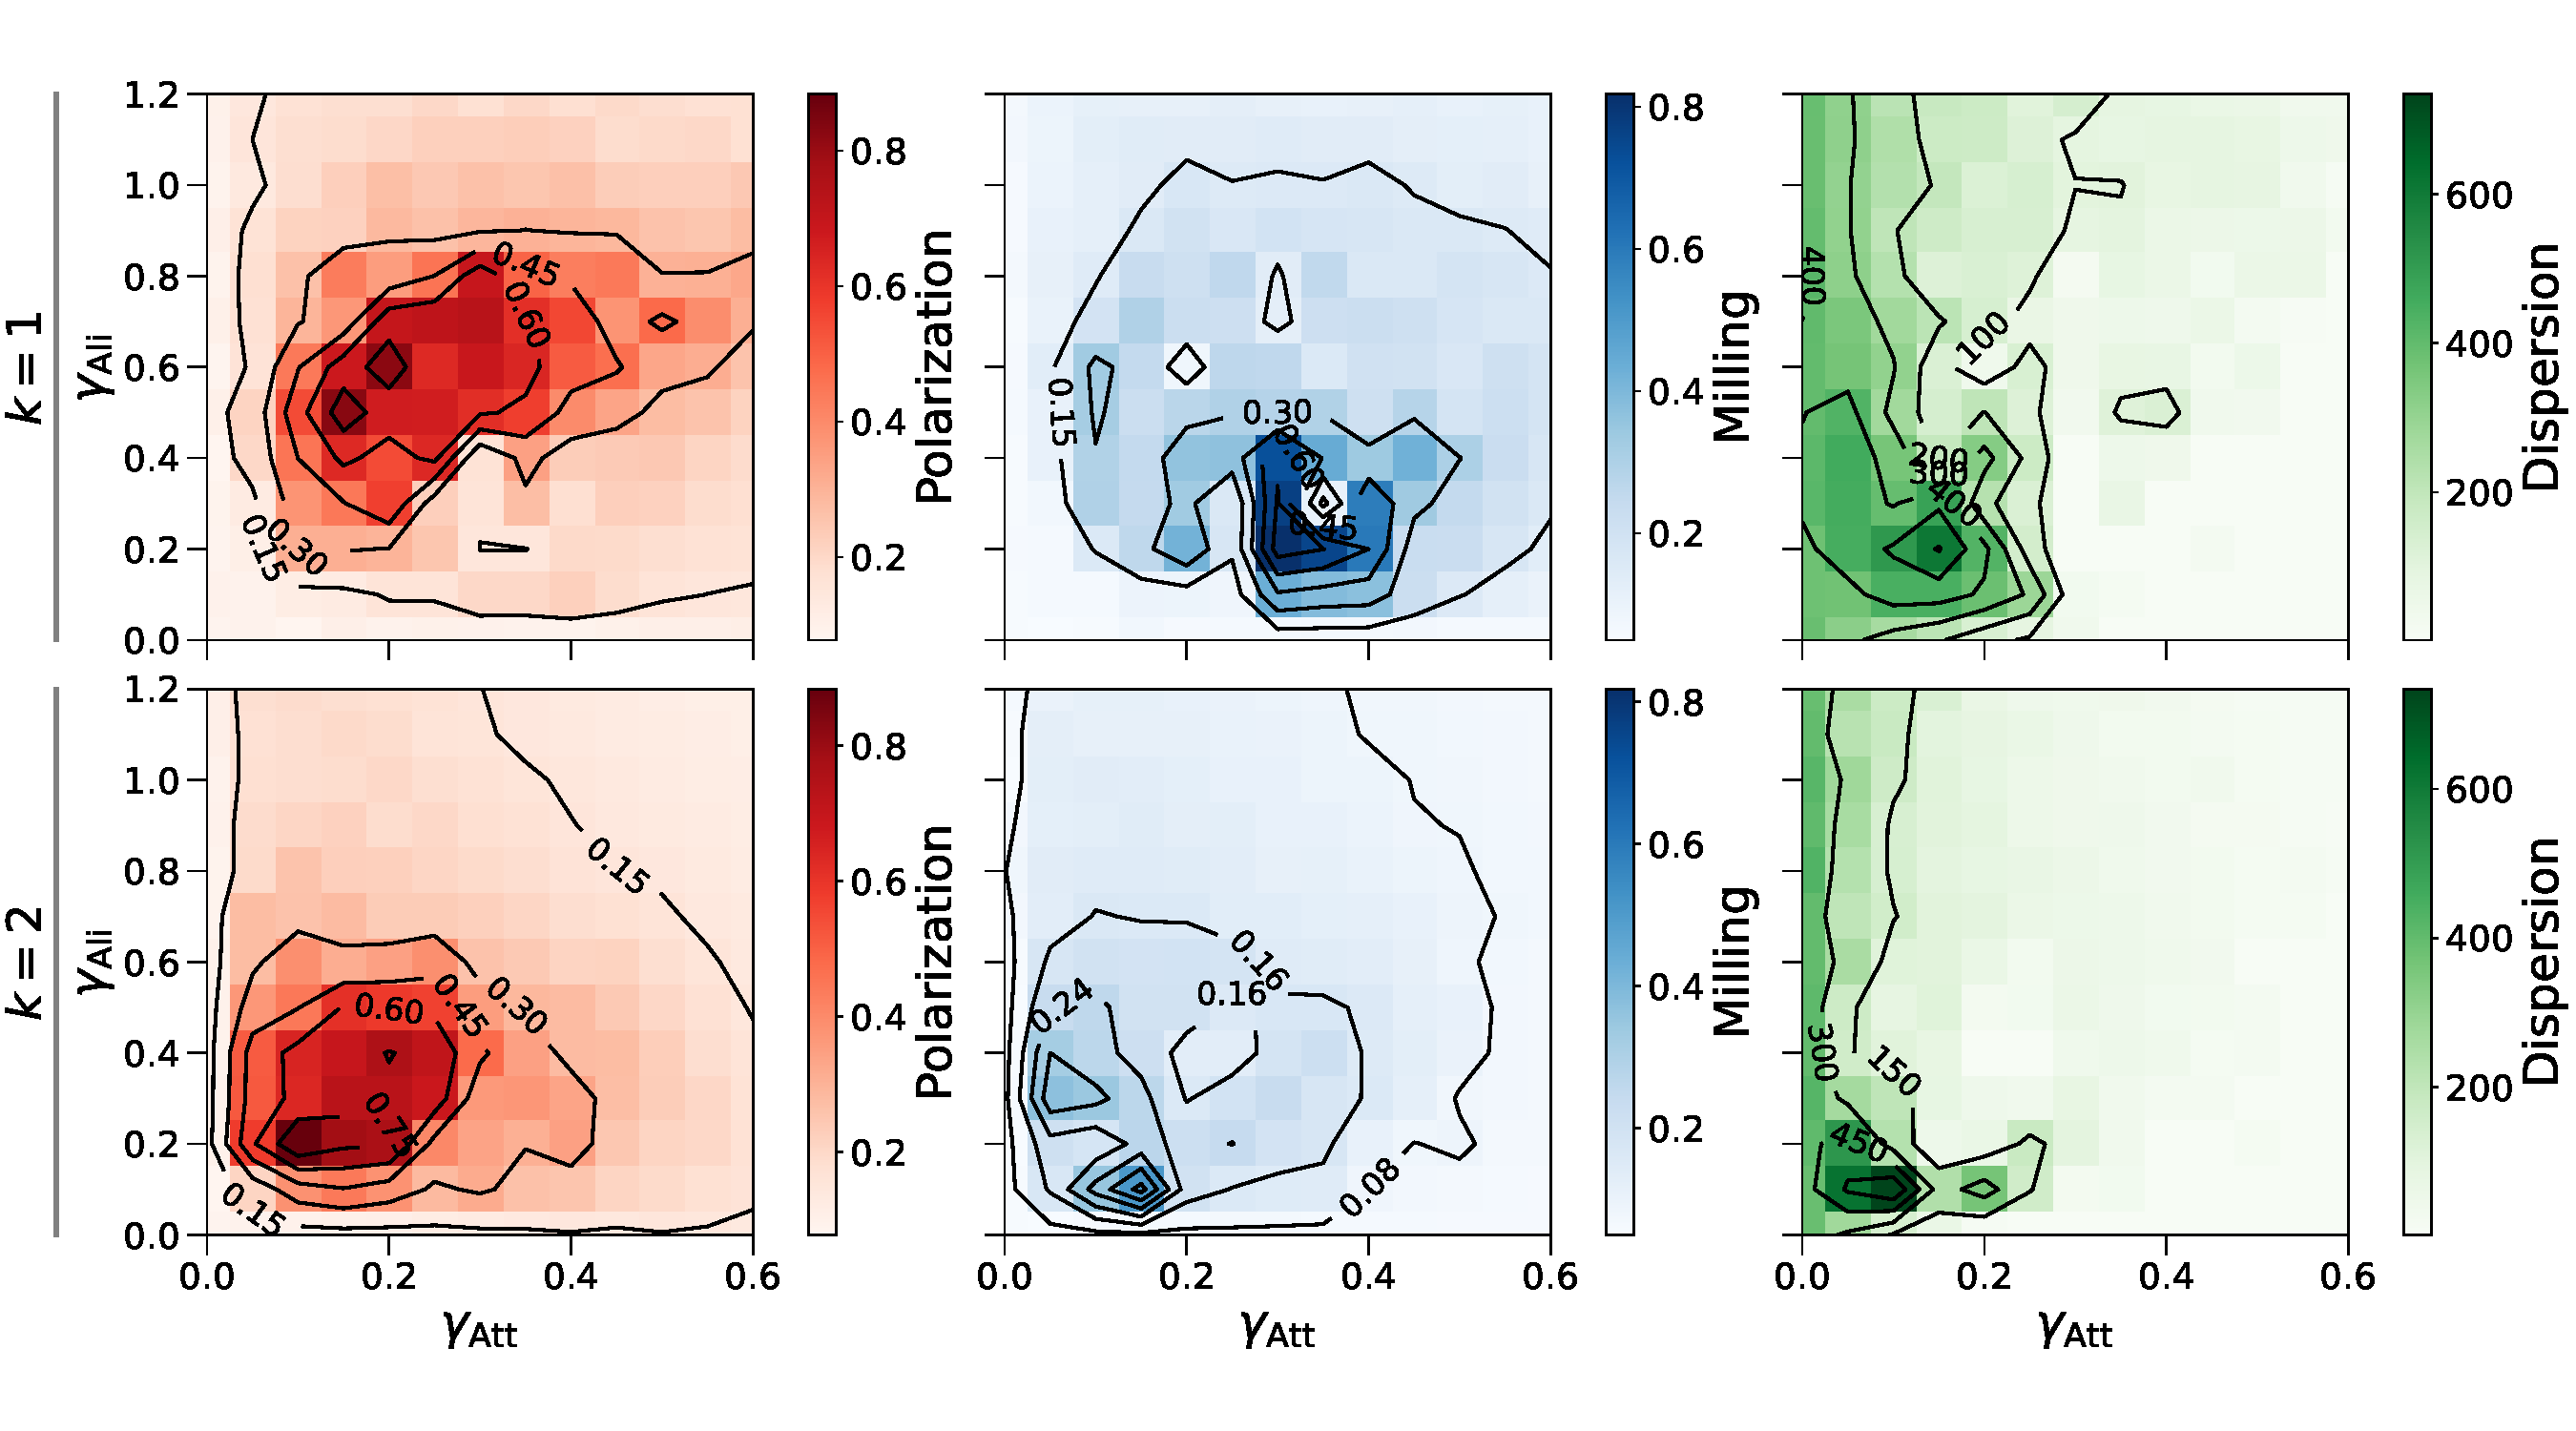
\includegraphics[width=1.0\linewidth]{figures/extended_model/combined_omega=00_nomega=1.pdf}
    \caption{Extended model with $\omega = 0$ and $n_\omega = 1$, which reproduces the base implementation. The dispersion color bar spans values up to 600, indicating that the school is highly spread out and frequently fragmented. Shown are polarization (red), milling (blue), and dispersion (green) for different combinations of attraction strength ($\gamma_{\mathrm{Att}}$), alignment strength ($\gamma_{\mathrm{Ali}}$), and number of influential neighbors ($k$). Each data point is averaged over 20 independent runs with different random seeds, where each run lasts $2000 \times N = 200{,}000$ kicks. Metrics are collected only after the first $1000 \times N$ kicks to reduce the influence of initial conditions.}
    \label{fig:w0nw1}
\end{figure}


%%%%%%%%%%%%%%%%%%%%%%%%%%%%%%%%%%%%%%%%%%%%%%%%%%%%%%%%%%%%%%%%%%%%%%%%%%%%%%%%%

\begin{figure}[!h]
    \centering
    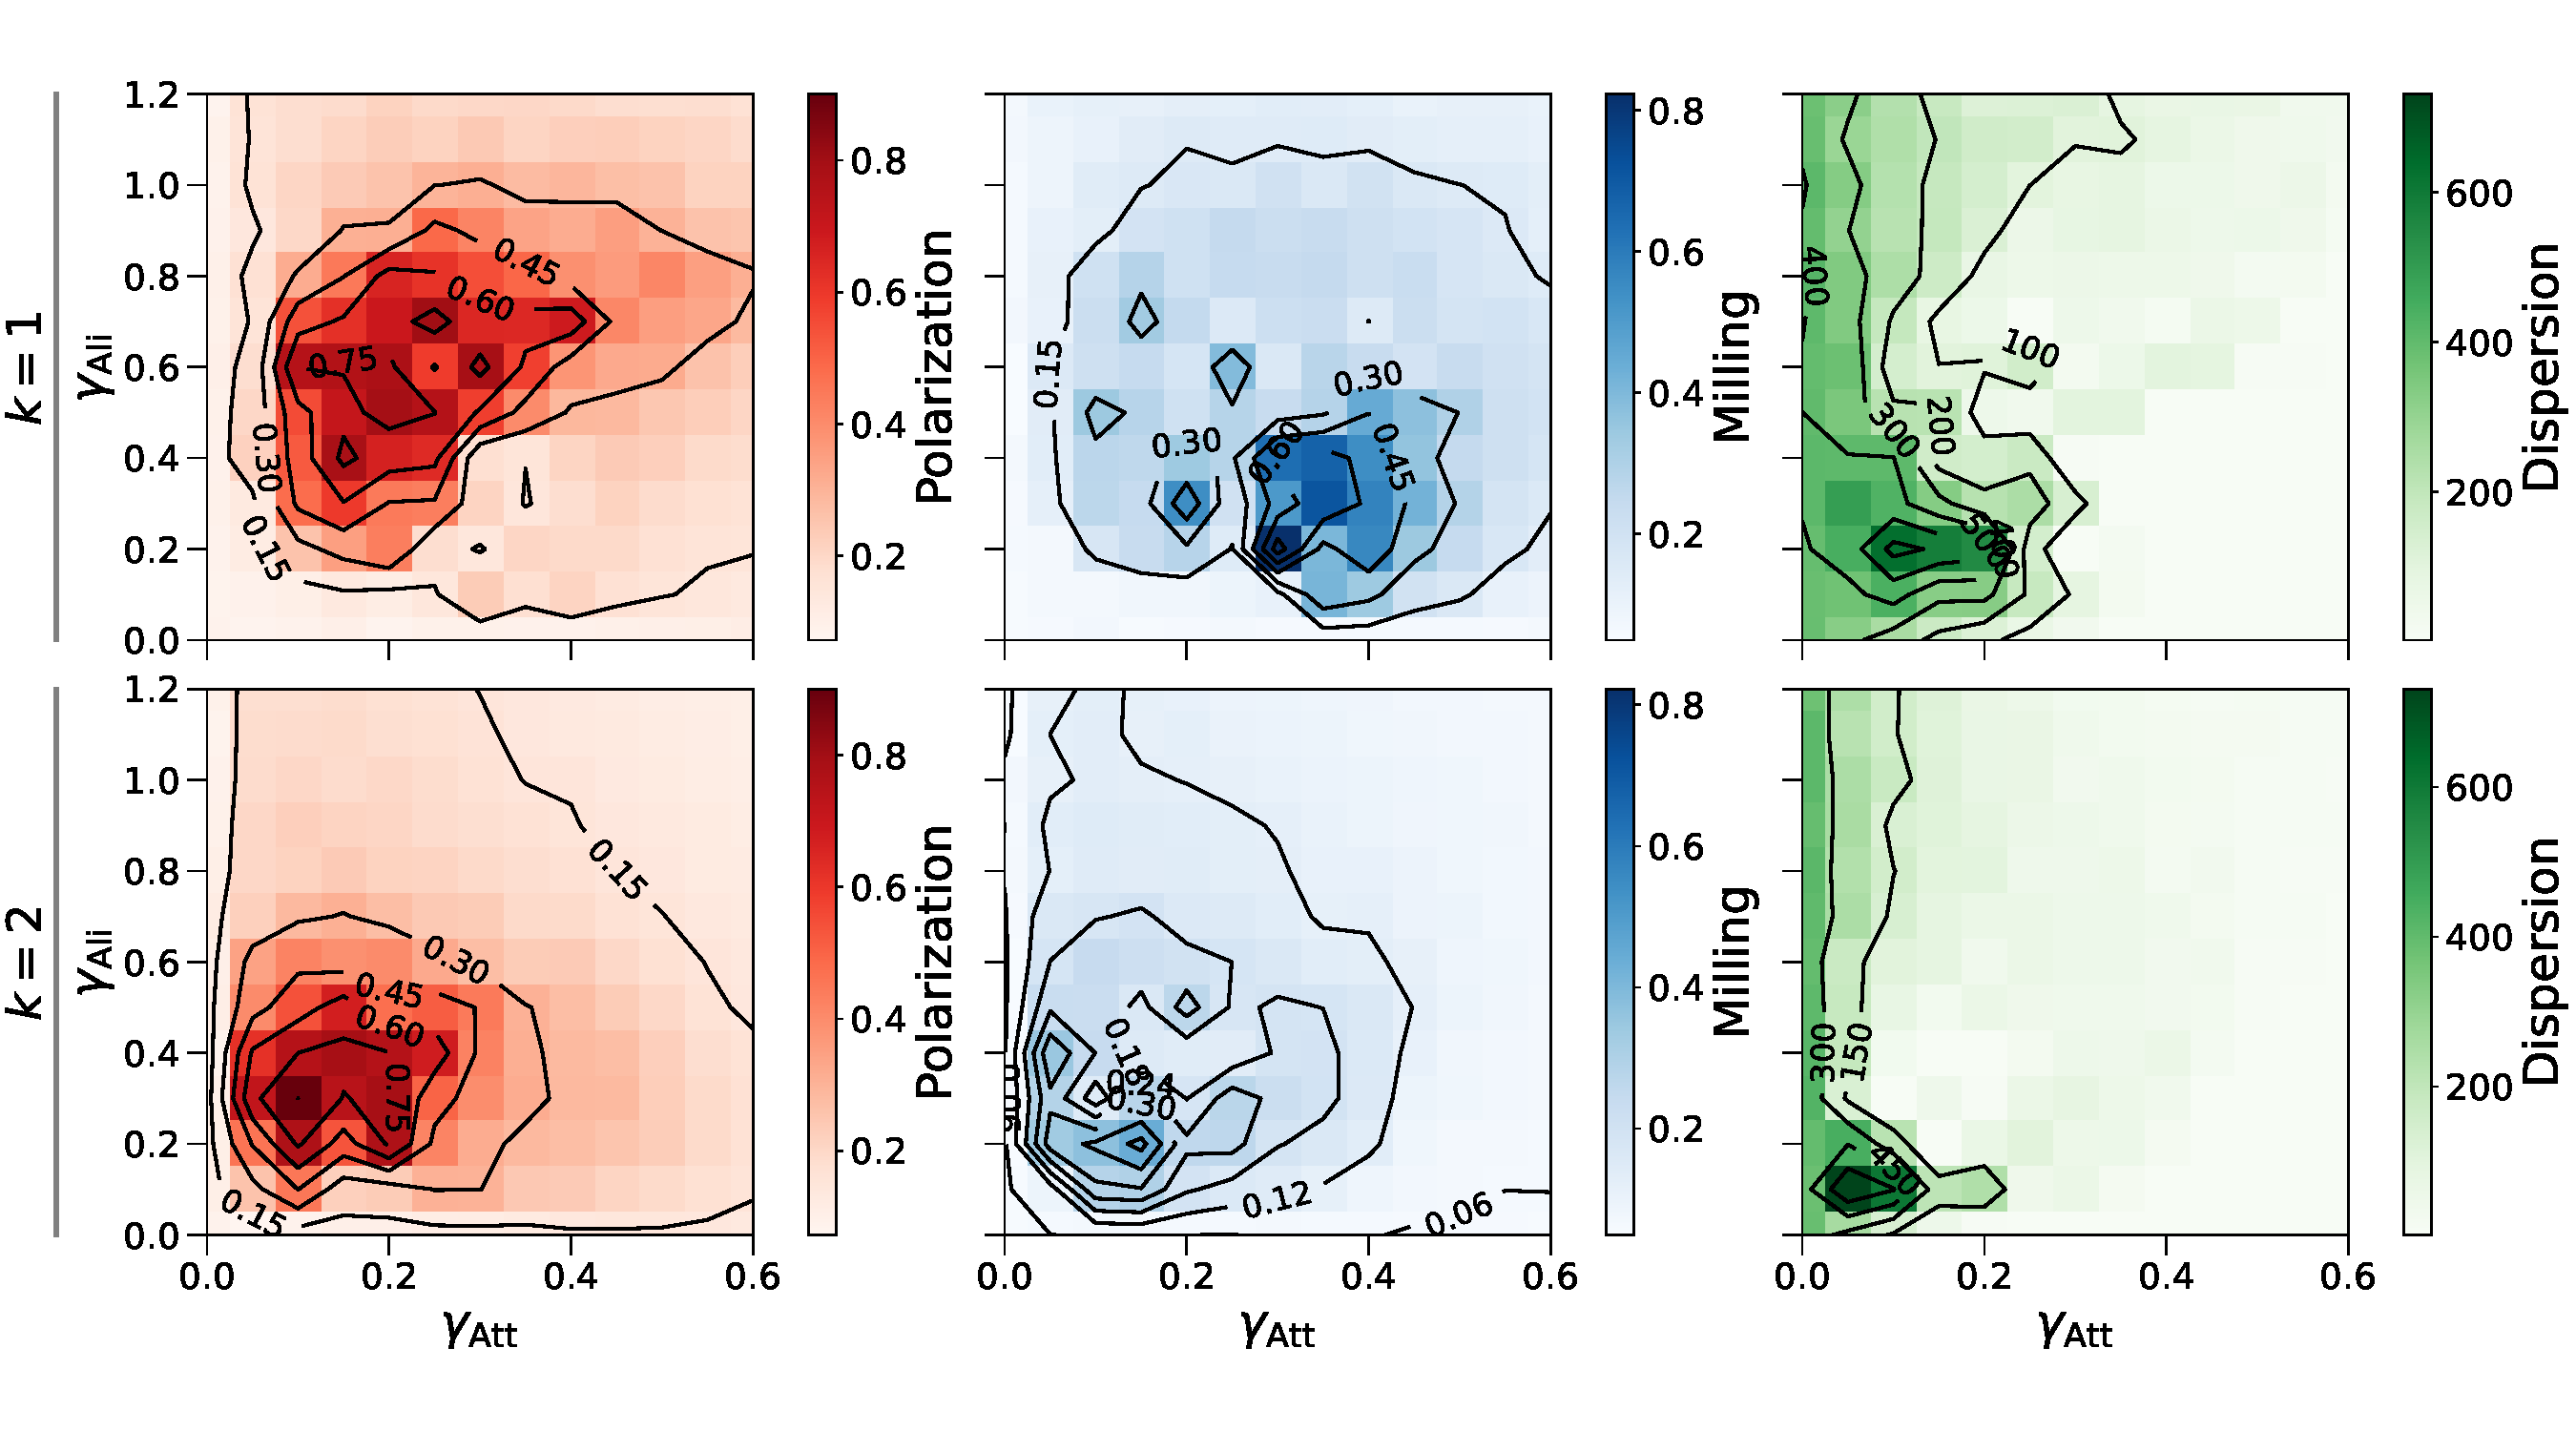
\includegraphics[width=1.0\linewidth]{figures/extended_model/combined_omega=05_nomega=1.pdf}
    \caption{Extended model with $\omega = 0.5$ and $n_\omega = 1$. Polarization is slightly higher compared to the base implementation, as indicated by the emergence of a $0.75$ polarization contour. The central milling region is marginally more spread out. However, due to the low decision resolution ($n_\omega = 1$), these differences remain minor, and the school overall remains unstable and prone to fragmentation.}
    \label{fig:w05nw1}
\end{figure}

%%%%%%%%%%%%%%%%%%%%%%%%%%%%%%%%%%%%%%%%%%%%%%%%%%%%%%%%%%%%%%%%%%%%%%%%%%%%%%%%%

\begin{figure}[!h]
    \centering
    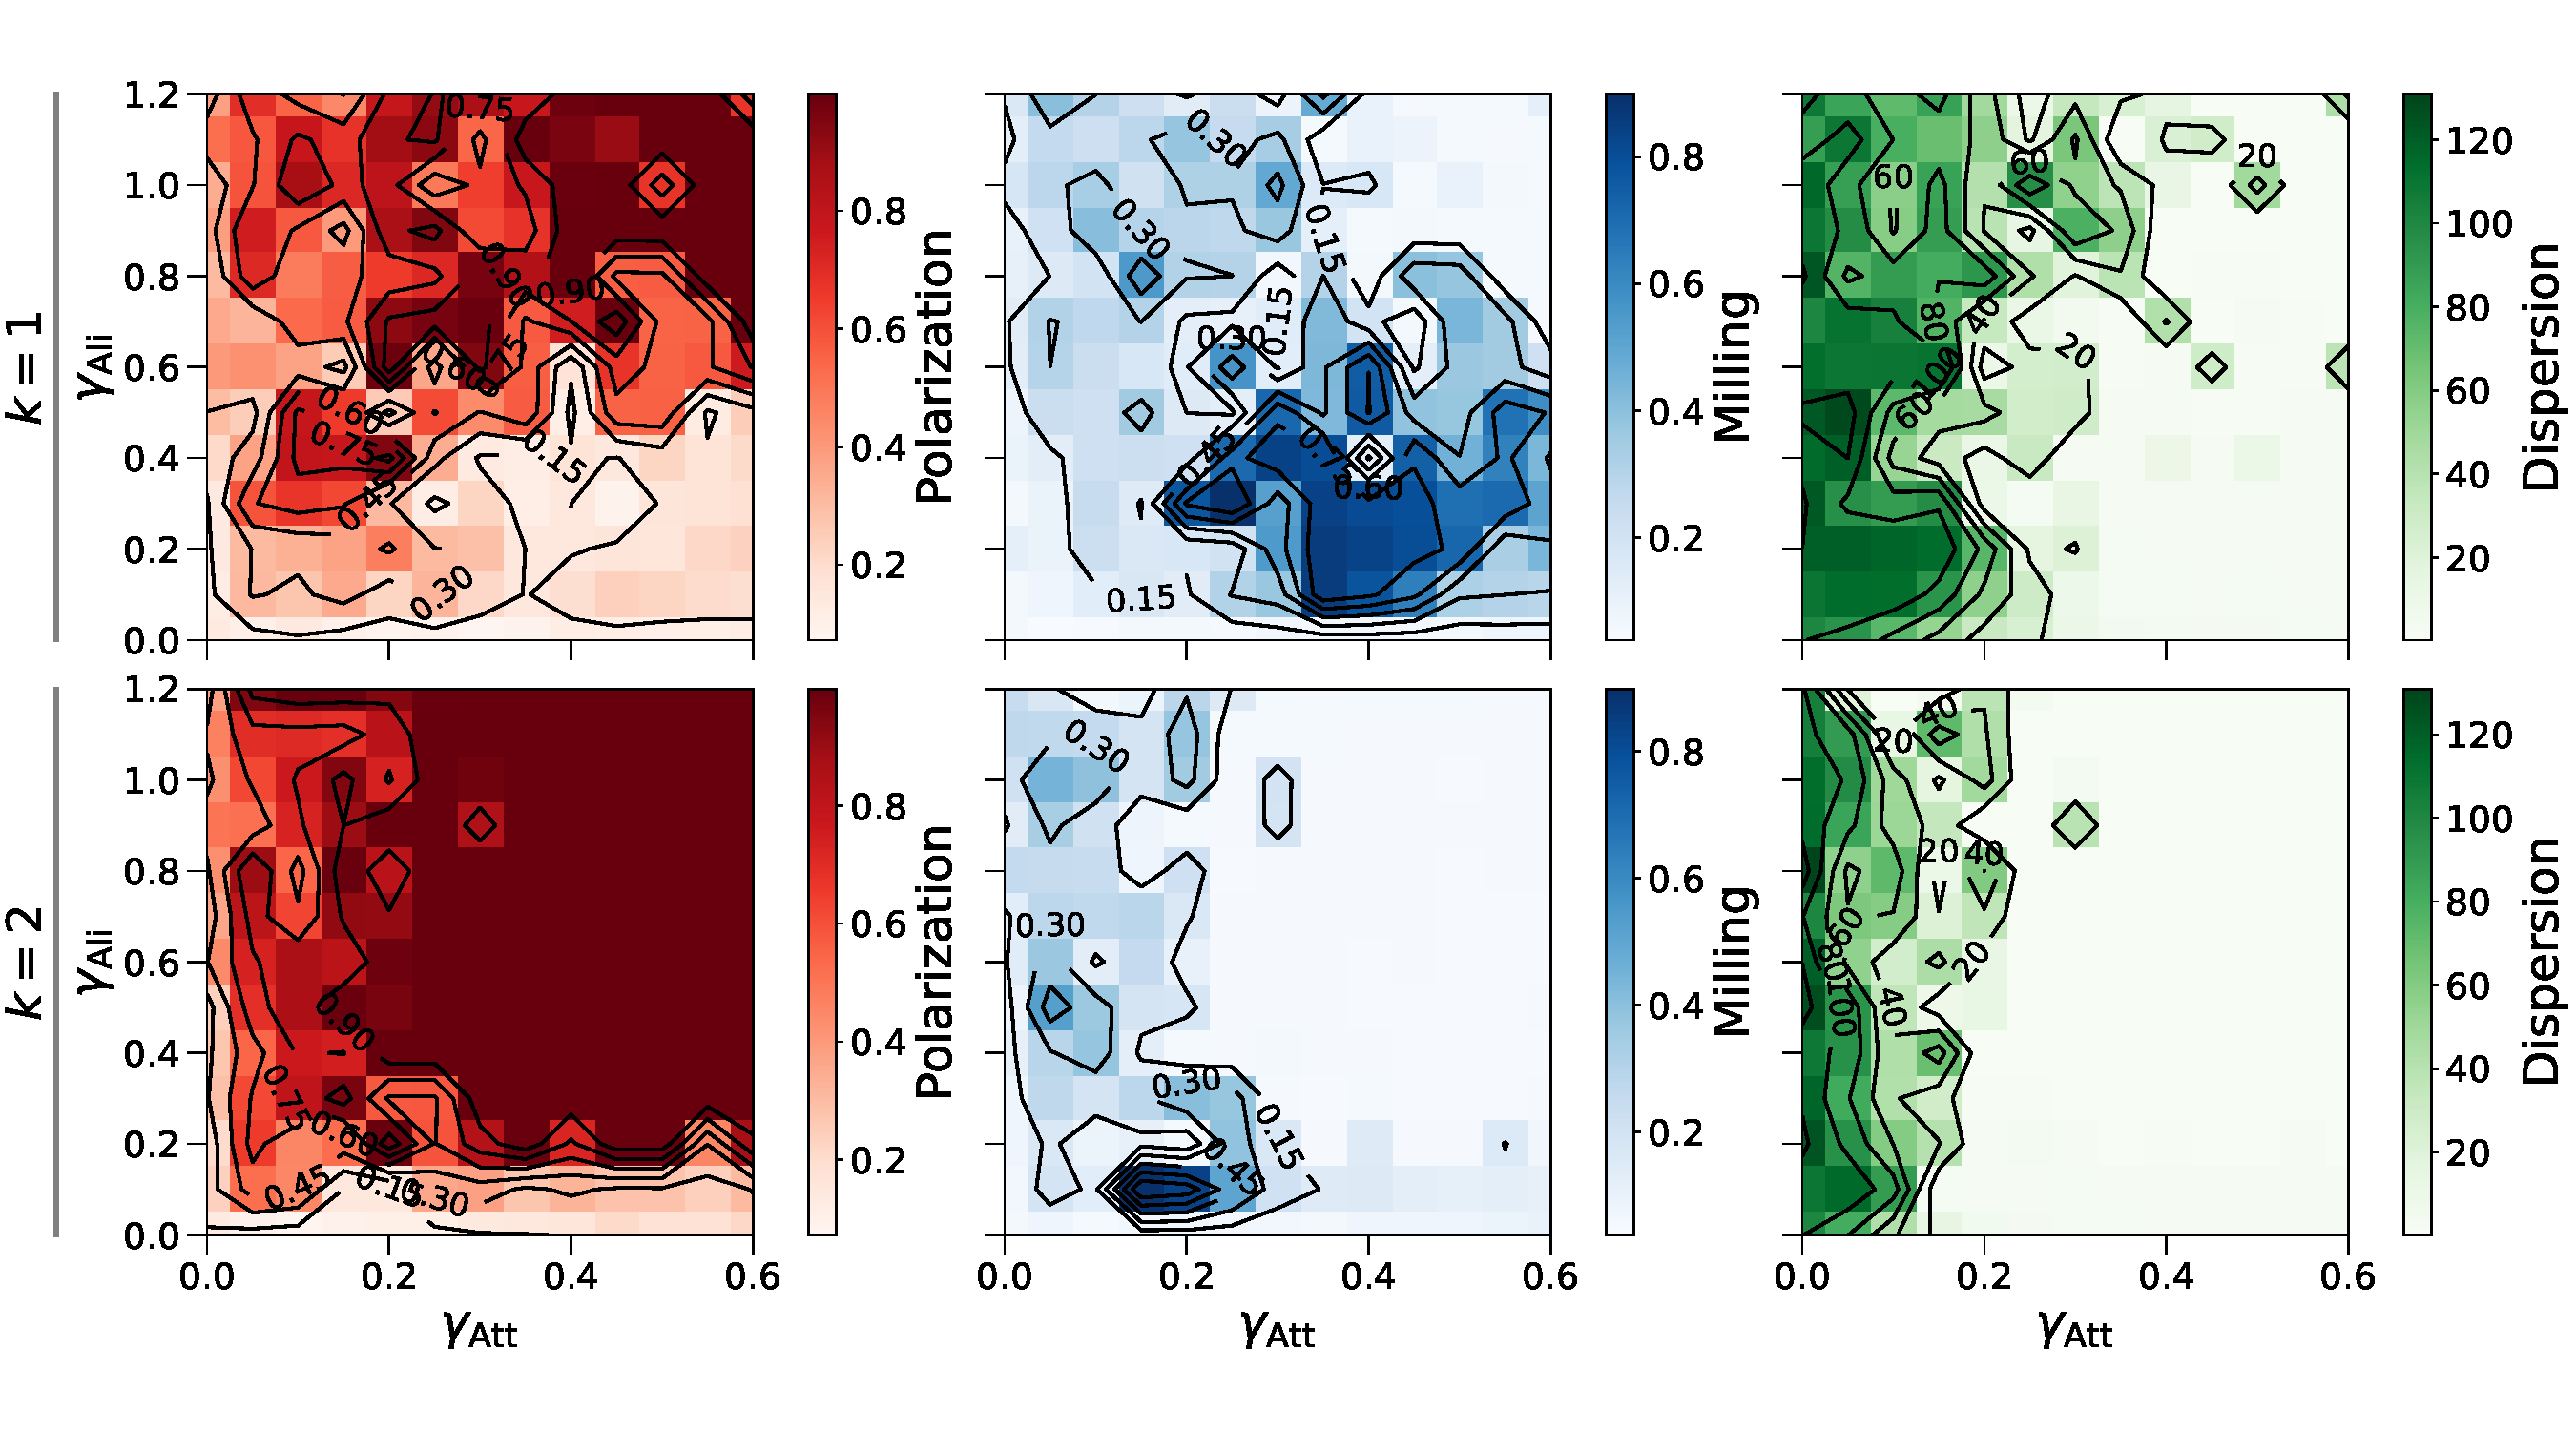
\includegraphics[width=1.0\linewidth]{figures/extended_model/combined_omega=00_nomega=10.pdf}
    \caption{Extended model with $\omega = 0$ and $n_\omega = 10$. Increasing the number of decision steps leads to a significantly more compact and cohesive school, with dispersion values reaching approximately 120 instead of 600. The increased presence of dark green regions reflects the rescaled color bar rather than higher absolute dispersion. Polarization is markedly stronger, as indicated by extended dark red regions, showing that fish are nearly parallel. Strong milling states (dark blue) emerge, demonstrating the ability of the school to maintain stable circular motion without tangential escape.}

    \label{fig:w0nw10}
\end{figure}


%%%%%%%%%%%%%%%%%%%%%%%%%%%%%%%%%%%%%%%%%%%%%%%%%%%%%%%%%%%%%%%%%%%%%%%%%%%%%%%%%

\begin{figure}[!h]
    \centering
    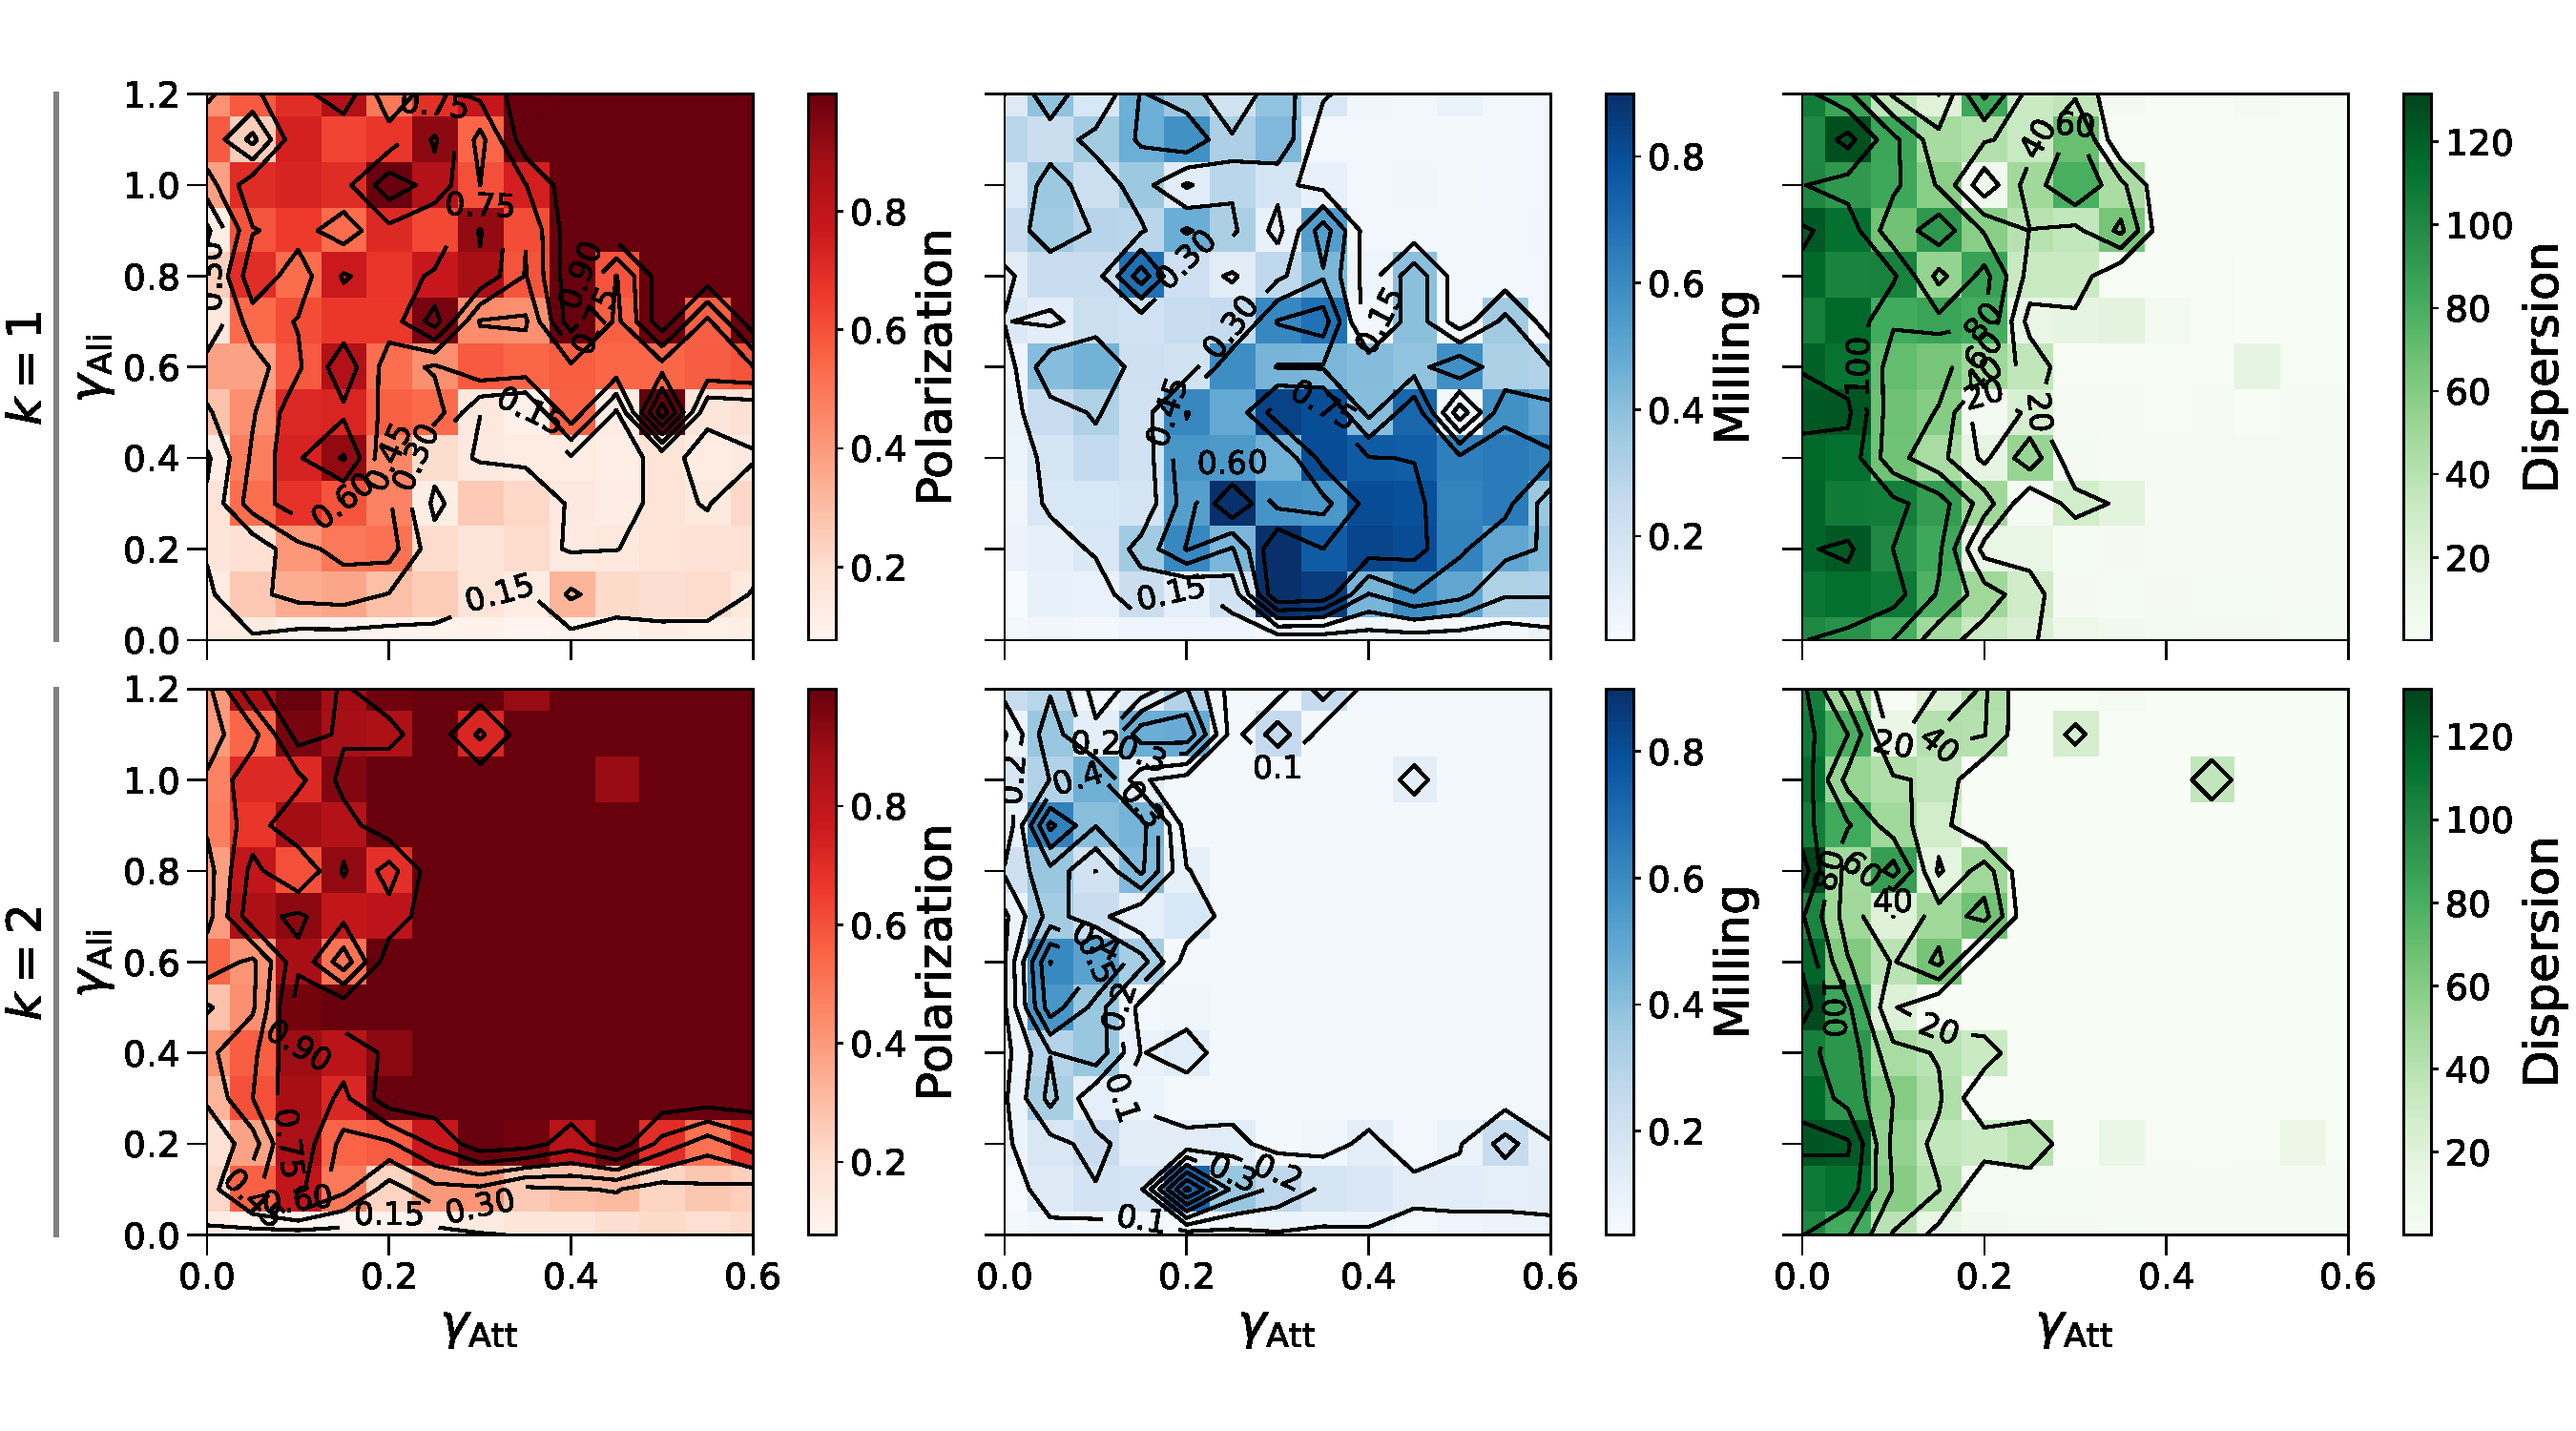
\includegraphics[width=1.0\linewidth]{figures/extended_model/combined_omega=05_nomega=10.pdf}
    \caption{Extended model with $\omega = 0.5$ and $n_\omega = 10$. The polarized region (red) is slightly larger and more contiguous compared to lower $\omega$, indicating that the school becomes locked into a parallel formation. In this regime, alignment emerges partly from kinematic persistence in addition to social interactions. Milling is moderately suppressed, as evidenced by weaker and more diffuse peaks, consistent with sustained speed causing agents to overshoot circular trajectories. Dispersion is slightly reduced compared to the $\omega = 0$ case at the same $n_\omega$, suggesting that while $n_\omega$ primarily governs cohesion, sustained propulsion further enhances dynamic coupling within the school.}

    \label{fig:w05nw10}
\end{figure}


